\documentclass[12pt,english,aspectratio=169]{beamer}
\usepackage[english]{babel}
\usepackage[T1]{fontenc}
\usepackage[latin2]{inputenc}

\usepackage{amstext}
\usepackage{amsthm}
\usepackage{amssymb}
\usepackage{amsmath}


\usepackage{booktabs}

\definecolor{sarga}{HTML}{FFAA55}
\definecolor{lila}{HTML}{C92AD5}
\definecolor{kek}{HTML}{0100FF}

\usetheme{Warsaw}
\useoutertheme{infolines}

\setbeamertemplate{headline}{}
%\setbeamerfont{page number in head/foot}{size=\tiny}
%\setbeamertemplate{footline}[frame number]

\setbeamersize{text margin left=0.5cm}
\setbeamersize{text margin right=0.5cm}
\setbeamertemplate{navigation symbols}{}

\title[Capstone Project]{Applied Data Science Capstone}
\subtitle{Where to open a new office in Budapest}
\date[2021]{\today}
\author[Norbert Bogya]{Norbert Bogya\\{\small\href{bnorbert88@gmail.com}{bnorbert88@gmail.com}}}




\begin{document}
\maketitle

\begin{frame}{Business Problem}
	When a \alert{new start-up IT company} levels up and can afford a real \alert{office} instead of working home, it is quite important to \alert{open} it in as suitable neighbourhood as possible.\bigskip
	
	Parameters, should be considered:
	\begin{itemize}
		\item renting price
		\item size and scalability of the office
		\item human factors
	\end{itemize}\bigskip

	Ideal spot: youthful neighbourhood near university buildings that provide a motivating working environment.
\end{frame}

\begin{frame}{Considered human factors}
	\begin{itemize}
		\item To create a \alert{motivating} working environment, a \alert{dynamic office-block area} is needed to choose. If workers are surrounded by similar workers, who enjoys to work there, it will help their productivity.\medskip
		\item As the potential \alert{new workers} will come from the \alert{universities} of Budapest, it is convenient to find a place that is near the main university buildings and colleges. In this case it will be much more attractive for young, agile students who are taking classes at a university in parallel their job.\medskip
		\item To increase the \alert{youthfulness} of the area, it is recommended to choose a neighbourhood with places that are preferred in the circle of young people. For example, \alert{caf�s} in the area will empower the attractiveness among them.
	\end{itemize}
\end{frame}

\begin{frame}{Goal}
	We try to cluster the neighbourhoods in Budapest, considering the number of existing office buildings, university buildings and caf�s, and with the help of this clustering to provide a suggestion to the spot that is suitable for a new office.
\end{frame}

\begin{frame}{Data: Wikipedia page about the neighbourhoods of Budapest}
	\framesubtitle{\url{https://hu.wikipedia.org/wiki/Budapest_v\%C3\%A1rosr\%C3\%A9szeinek_list\%C3\%A1ja}}
	
	Budapest is divided onto 23 districts, and each district may contain several neighbourhoods. We use only the ``N�v'' and ``Ker�let'' columns of the table, which correspond to the names of the \alert{neighbourhoods} and \alert{districts}, respectively.
	\begin{center}
		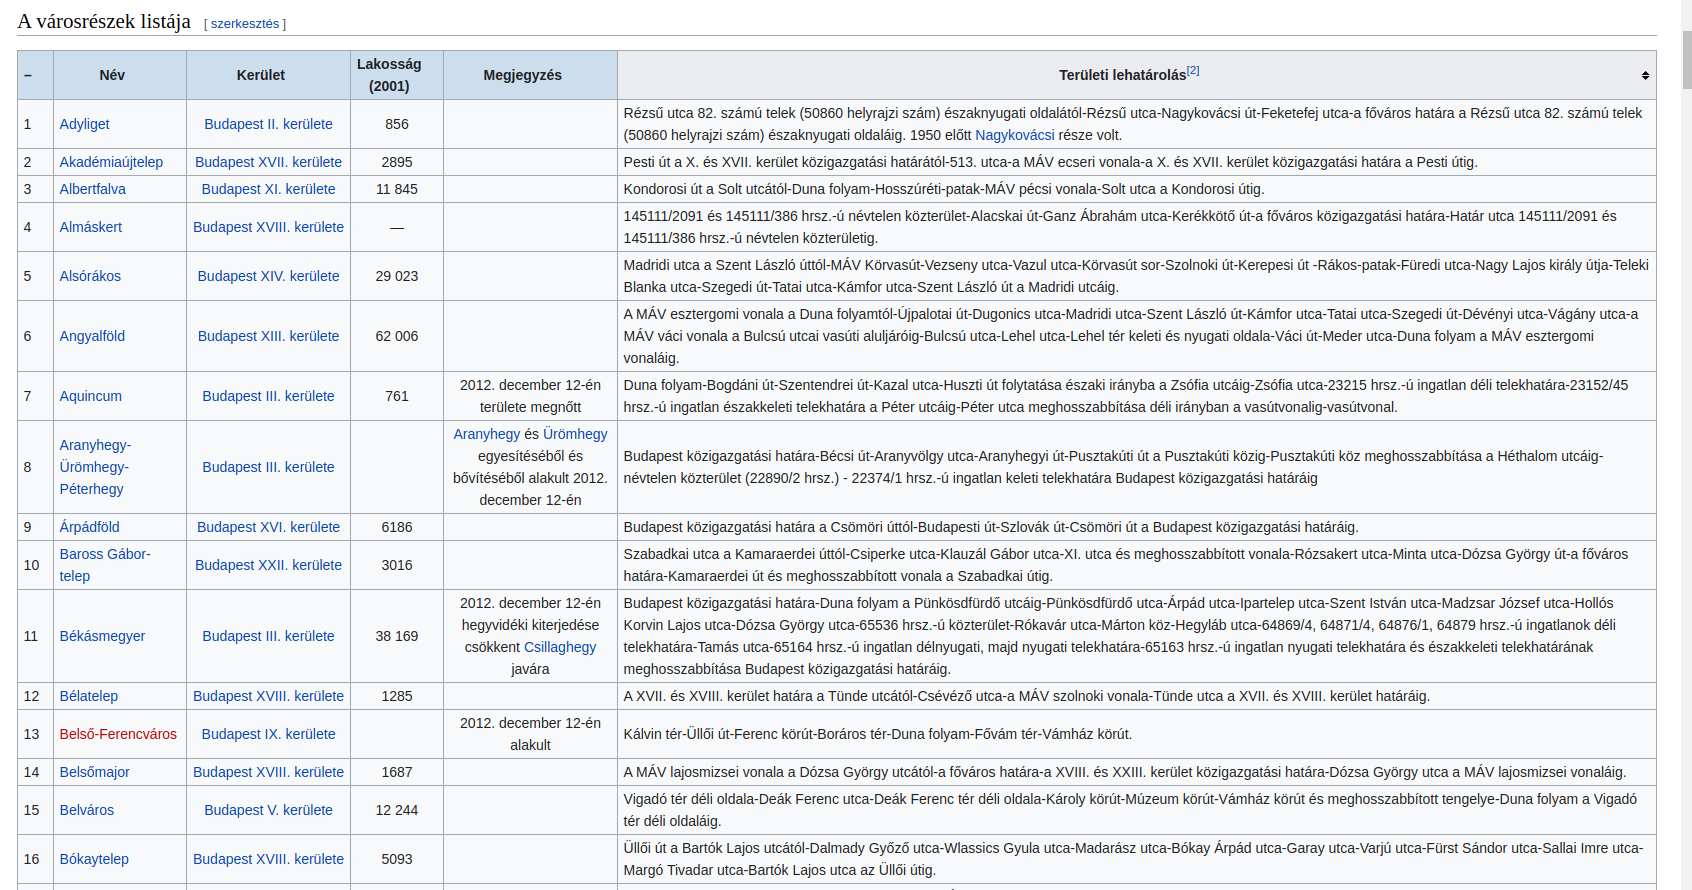
\includegraphics[width=1\linewidth]{neighbourhoods}
	\end{center}
\end{frame}

\begin{frame}{Data: \textit{Foursquare} API}
	\framesubtitle{\url{https://api.foursquare.com}}
	We use the \textit{Foursquare} API the explore the venues of areas.
	\begin{center}
		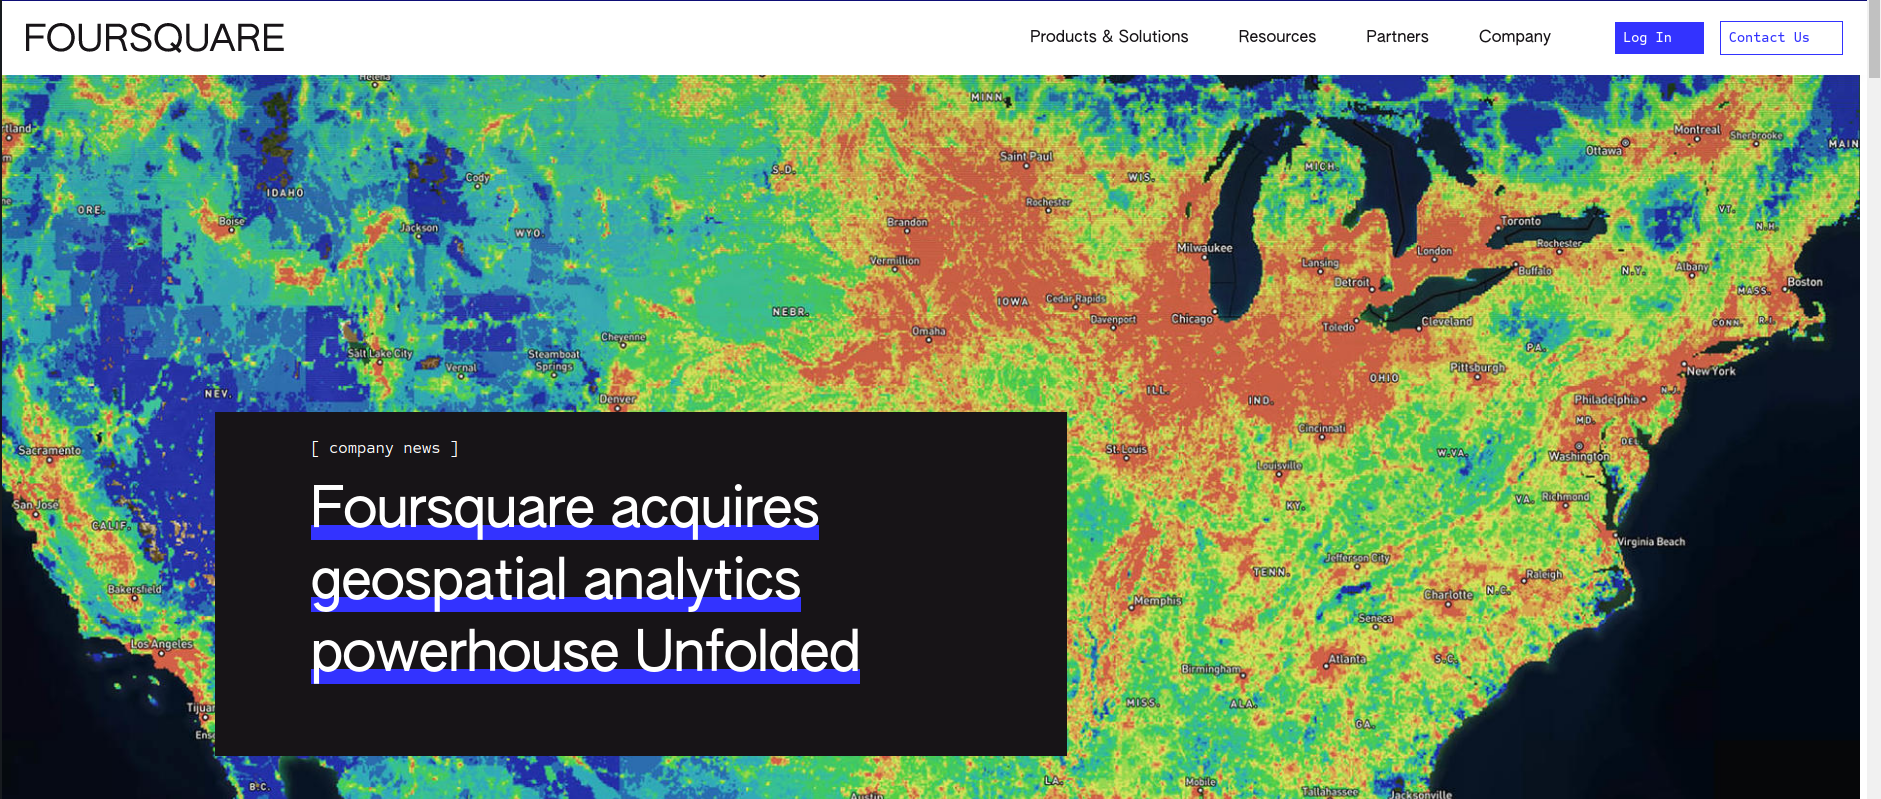
\includegraphics[width=1\linewidth]{foursquare}
	\end{center}
\end{frame}

\begin{frame}
	During the API calls, we filters for the mentioned categories of the venues: \alert{caf�s, universities and offices}. Foursquare API has an option to restrict our exploration to several type of venues.
	\begin{center}
		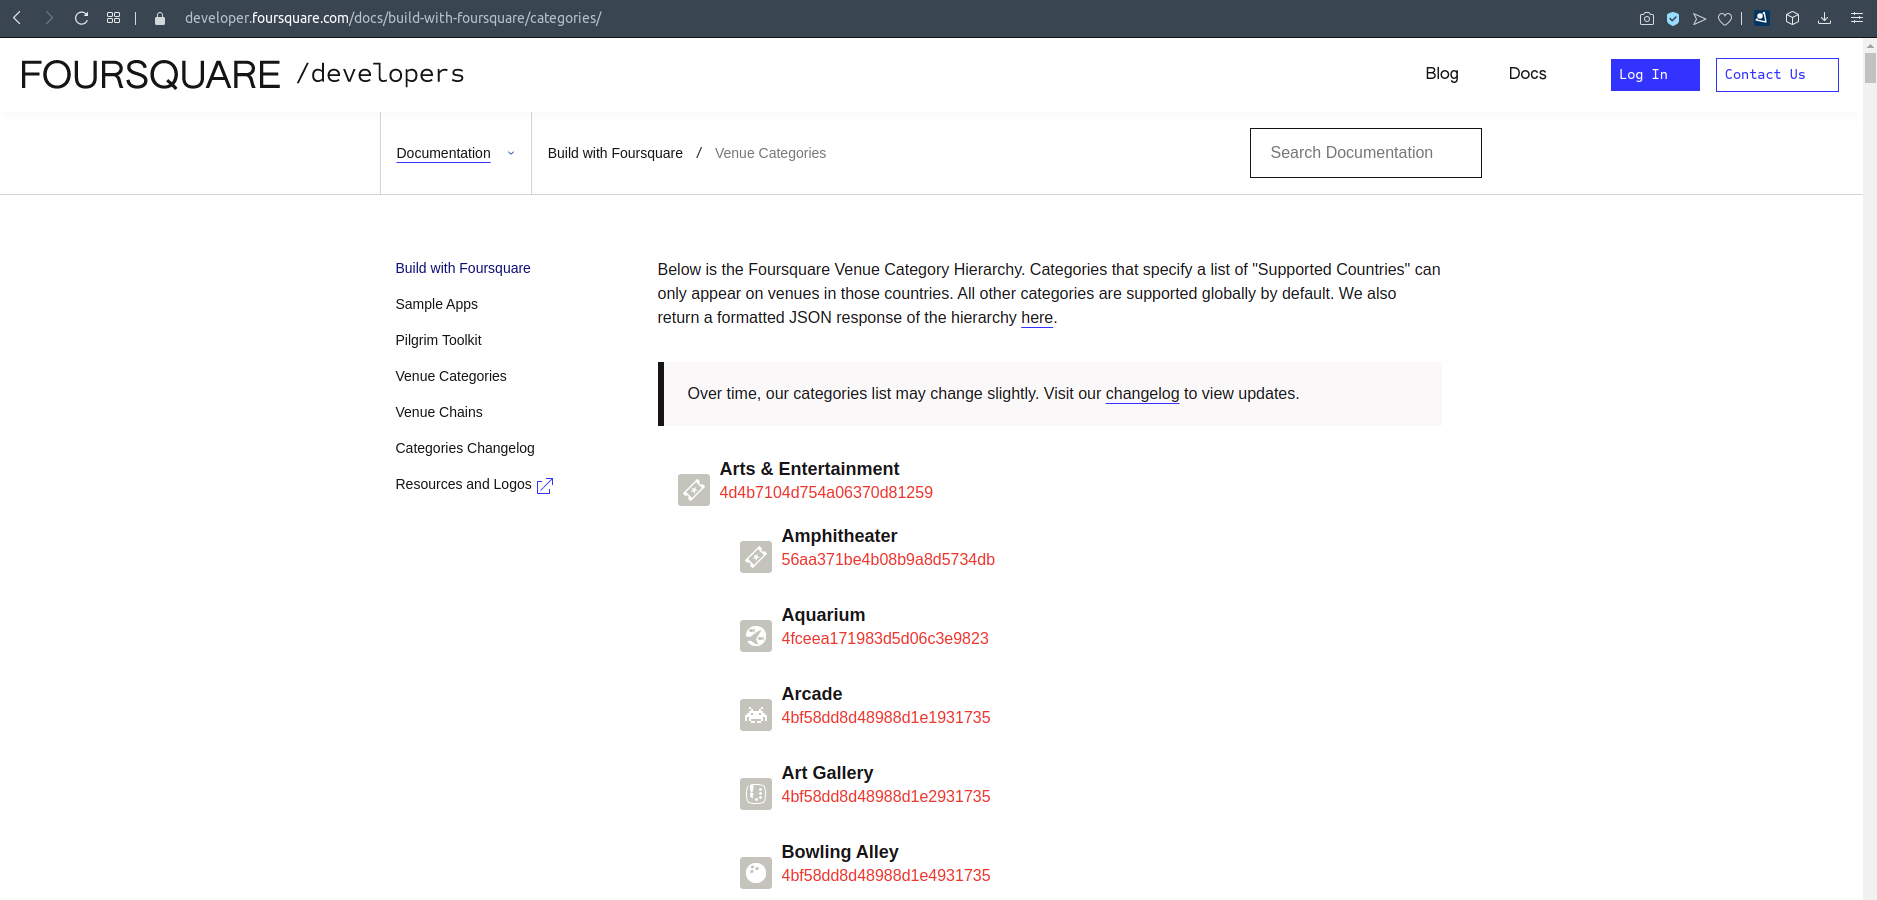
\includegraphics[width=1\linewidth]{foursquare2}
	\end{center}
\end{frame}

\begin{frame}{Methodology}
	Data manipulation:
	\begin{itemize}
		\item Loading data from Wikipedia: \textit{Beautiful Soup} Python library
		\item Store data: \textit{pandas} dataframes
		\item Geographic locations of neighbourhoods: \textit{GeoPy} Python client with \textit{Nominatim} and \textit{Photon} geocoding services
		\item Venue information: Foursquare API calls
	\end{itemize}
	\hrulefill
	
	Clustering:
	\begin{itemize}
		\item $k$-means algorithm by the \textit{scikit-learn} Python package
		\item Elbow rule to choose the optimal value of $k$
		\item Plot data points on map: \textit{Folium} package
	\end{itemize}
\end{frame}

\begin{frame}{Dataframe after data manipulation}
	\begin{center}
		{\color{magenta}Beautiful Soup} $\Longrightarrow$ pandas $\Longrightarrow$ {\color{cyan}GeoPy} $\Longrightarrow$ {\color{brown}Foursquare}
	\end{center}
	\begin{center}
		\begin{tabular}{lllrrrrr}
			\toprule
			{} & {\color{magenta}district} &    {\color{magenta}neighborhood} &   {\color{cyan}Latitude} &  {\color{cyan}Longitude} &  {\color{brown}office} &  {\color{brown}university} &  {\color{brown}cafe} \\
			\midrule
			0 &        I &     Gell�rthegy &  47.492064 &  19.037200 &       4 &           3 &     3 \\
			1 &        I &  Krisztinav�ros &  47.496866 &  19.029776 &      17 &           5 &     7 \\
			2 &        I &           Tab�n &  47.491613 &  19.043169 &       2 &           1 &     3 \\
			3 &        I &             V�r &  47.495334 &  19.039546 &       3 &           4 &     8 \\
			4 &        I &       V�ziv�ros &  47.503719 &  19.039128 &       4 &           3 &     8 \\
			5 &       II &        Adyliget &  47.547550 &  18.938984 &       0 &           0 &     0 \\
			6 &       II &   Budakeszierd� &  47.542471 &  18.972903 &       0 &           0 &     0 \\
			7 &       II &       Budaliget &  47.567579 &  18.940664 &       0 &           1 &     0 \\
			8 &       II &        Csat�rka &  47.531525 &  19.002578 &       0 &           1 &     0 \\
			9 &       II &   Erzs�betliget &  47.561714 &  18.967558 &       0 &           0 &     0 \\
			\bottomrule
		\end{tabular}
	\end{center}
\end{frame}

\begin{frame}{Optimal value of $k$ for clustering}
	Creating models with $k=2,3,\ldots 20$, we get the following distortion plot.
	\begin{center}
		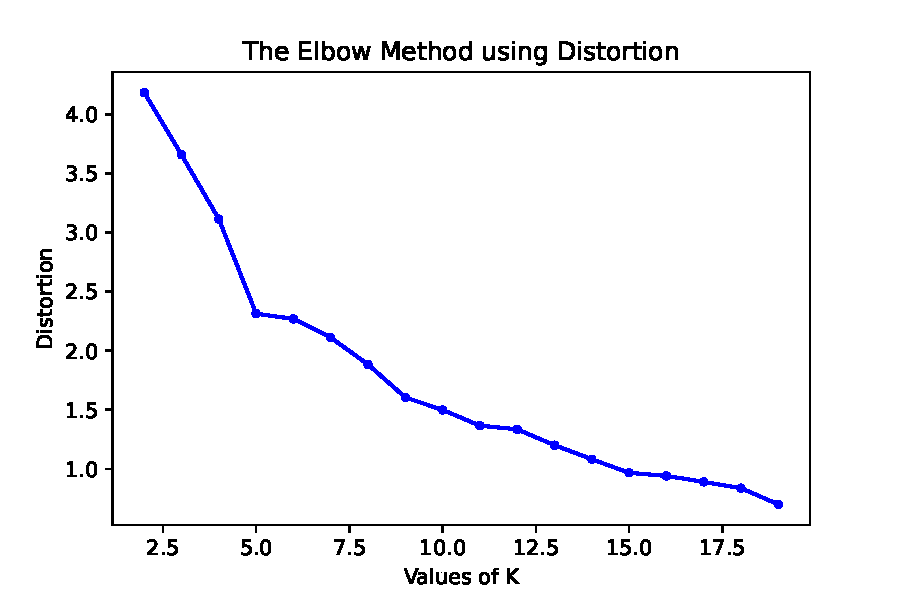
\includegraphics[width=0.5\linewidth]{kmeans}
	\end{center}
	Using the elbow method, we can see that the optimal choice for $k$ is 5.
\end{frame}

\begin{frame}{Clusters}
	Considering the number of caf�s, university and office buildings
	\begin{center}
		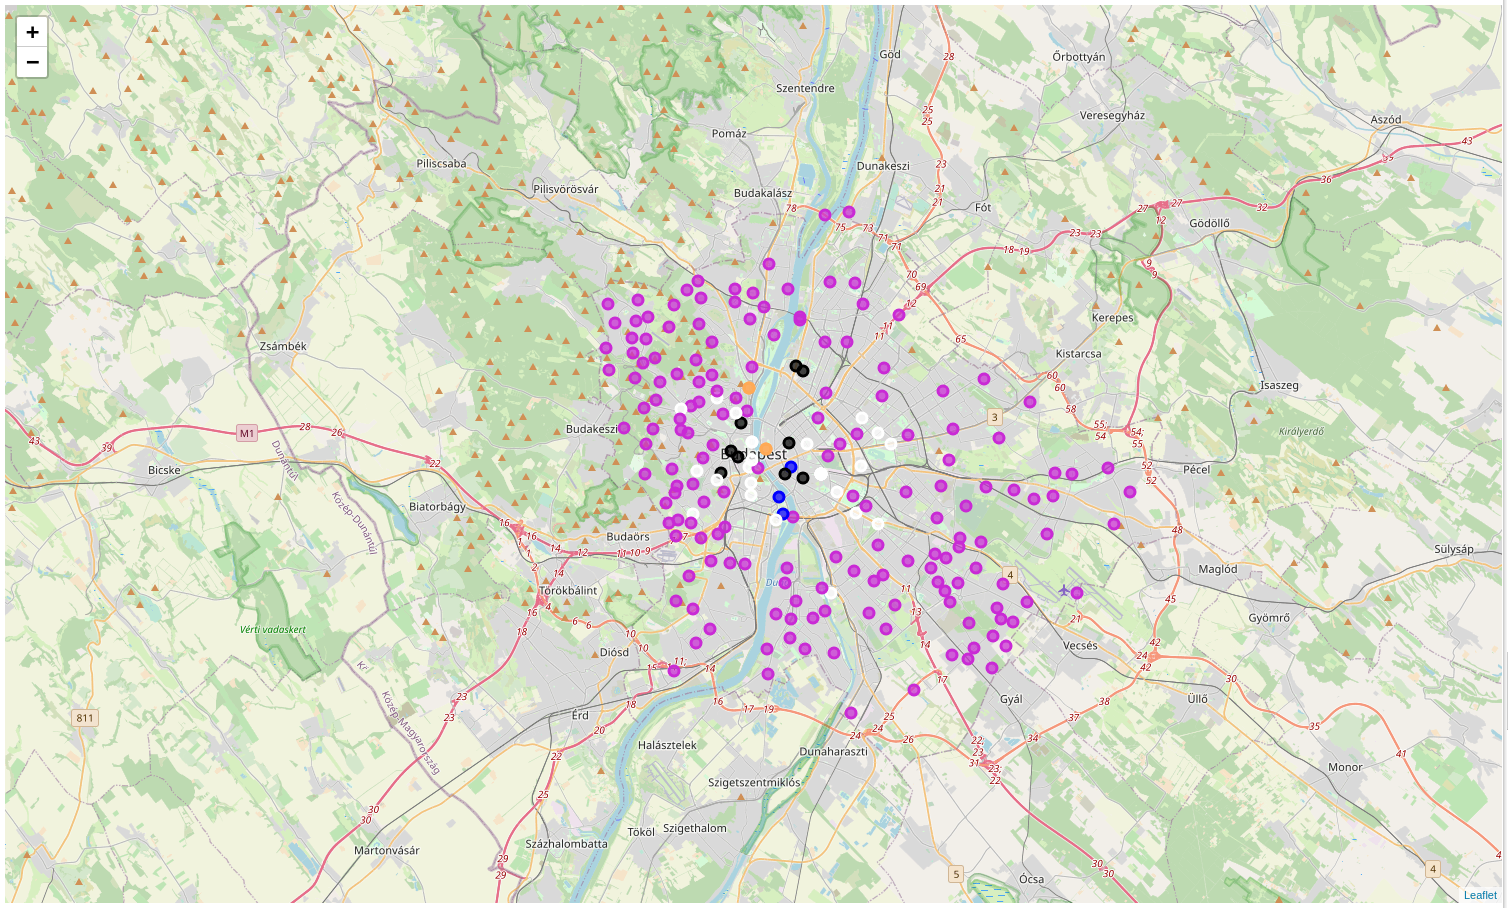
\includegraphics[width=1\linewidth,trim=160 150 160 200, clip]{bp2}
	\end{center}
\end{frame}

\begin{frame}{Size of clusters}
	\begin{center}
		\begin{tabular}{lr}
			\toprule
			{} &    Size \\
			Cluster Labels &      \\
			\midrule
			0              &   29 \\
			1              &    9 \\
			2              &    3 \\
			3              &  164 \\
			4              &    4 \\
			\bottomrule
		\end{tabular}
	\end{center}
\end{frame}

\begin{frame}{Cluster 3}
	\begin{itemize}
		\item Most of the neighbourhoods lie in this cluster.
		\item This {\color{lila}cluster} is the least suitable for us.
		\item Triplets (universities,caf�s,offices) have low numbers.
		\item \alert{None} of these neighbourhoods can be \alert{recommended} to open a new office.
	\end{itemize}
	\begin{center}
		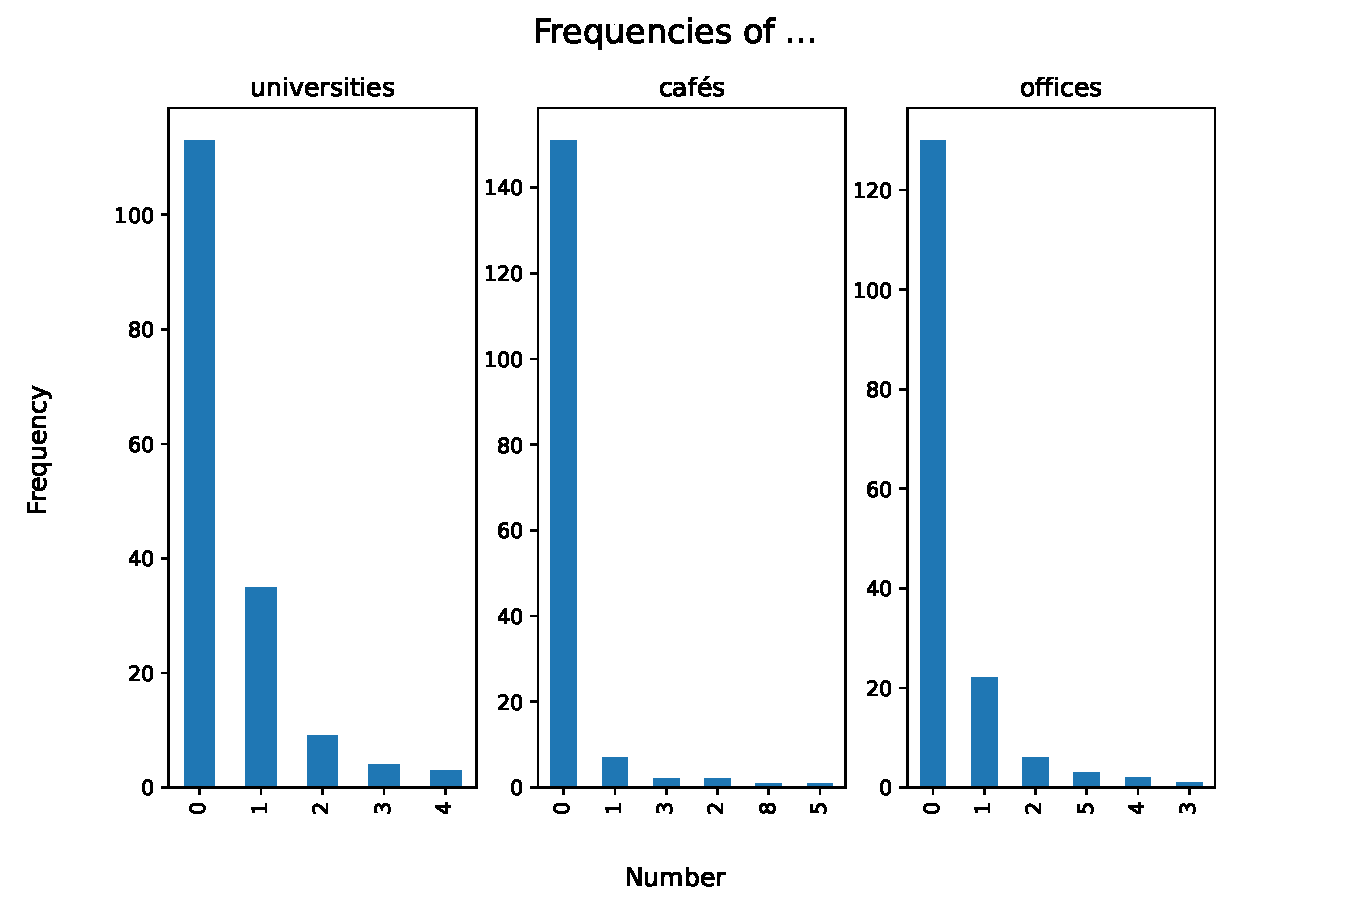
\includegraphics[width=0.5\linewidth]{df3}
	\end{center}
\end{frame}

\begin{frame}{Cluster 0}
	\begin{itemize}
		\item White dots.
		\item Few university buildings and quite small number of caf�s and universities.
		\item This cluster is \alert{neither recommended}, because of the small number of important factors.
	\end{itemize}
	\begin{center}
		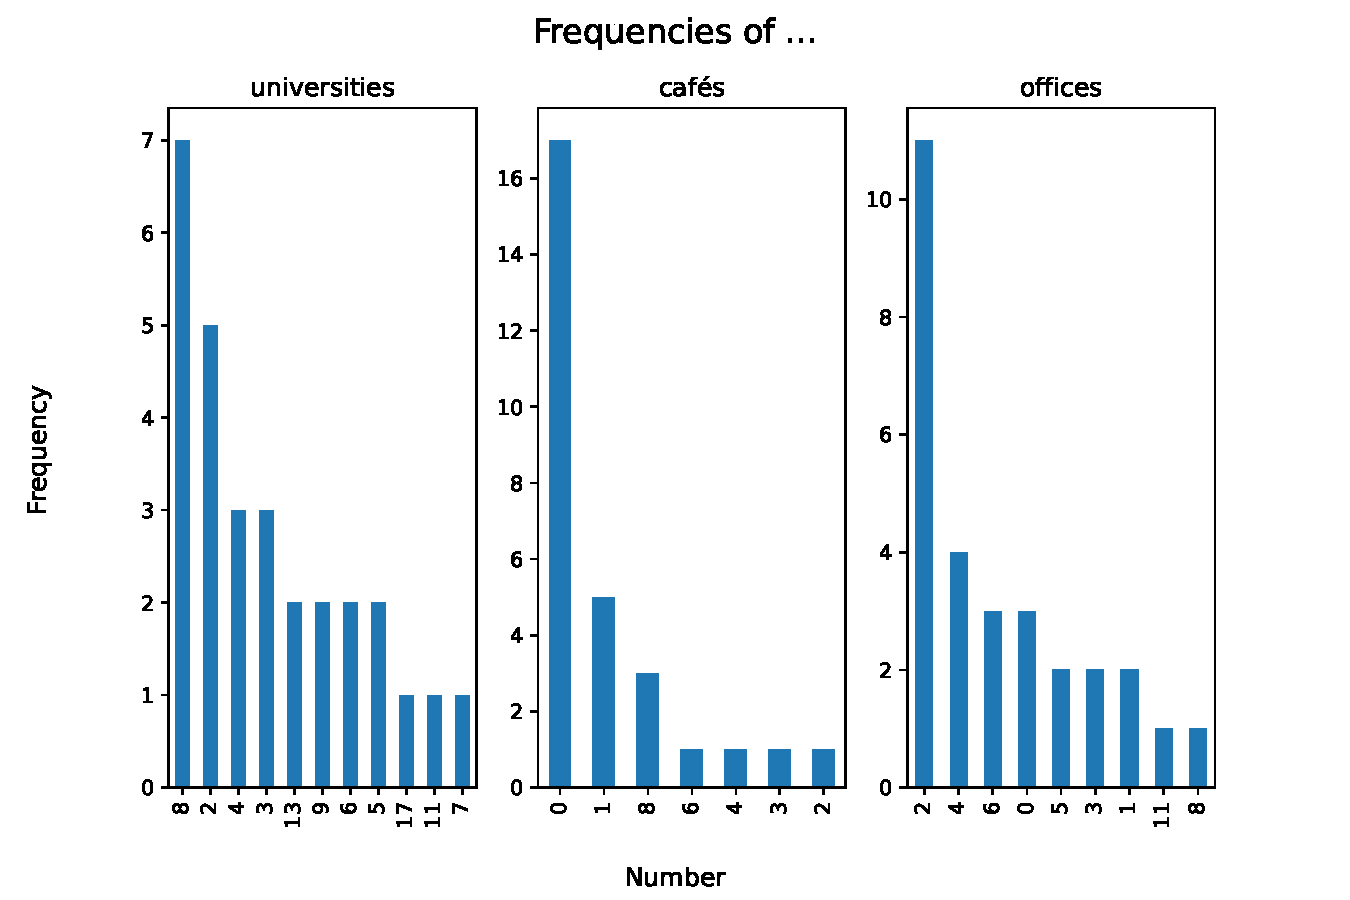
\includegraphics[width=0.5\linewidth]{df0}
	\end{center}
\end{frame}

\begin{frame}{Cluster 2}
	\begin{itemize}
		\item {\color{kek} Blue} dots.
		\item Only 3 elements.
		\item Large number of university buildings, however the number of offices and caf�s are quite small.
	\end{itemize}

	\hrulefill
	
	\begin{itemize}
		\item Main buildings of the two biggest universities of Budapest.
		\item Huge office area, called Infopark.
		\item Few number of reported caf�s, they are inside the universities and office buildings
		\item These spots are \alert{highly recommended to open new office}, but it is an overwhelmed area, and to open offices is not too cheap.
	\end{itemize}
\end{frame}

\begin{frame}{Cluster 1 and 4}
	\begin{itemize}
		\item {\color{sarga}\textbf{Cluster 4}} and {\color{black}\textbf{Cluster 1}} are similar clusters.
		\item Large number of office buildings but small number of caf�s and university buildings.
		\item Cluster 4 has only few element, and these neighbourhoods are the most crowded spots of Budapest, including the inner city. There are a lot of office buildings here, but they are far from the university campuses.
		\item Cluster 1 is more balanced with a lot of office building and moderate number of caf�s and university buildings.
		\item They can be recommended as a spot for a new office.
	\end{itemize}
\end{frame}

\begin{frame}{Conclusion}
	Taking everything into account, by this clustering method we can recommend the clusters in the following priority order.
	
	\begin{enumerate}
		\item Cluster 2
		\item Cluster 1
		\item Cluster 4
		\item Cluster 0
		\item Cluster 3
	\end{enumerate}
\end{frame}

\begin{frame}{End}
	\begin{center}
		Thank you for your attention!
	\end{center}
\end{frame}


\end{document}

